En este ejercicio vamos a mostrar los caracteres que se envíen a través del
puerto serie por un display LCD controlado desde la placa de Arduino. Para ello
las conexiones se dispondrán de la manera que se muestra aquí:

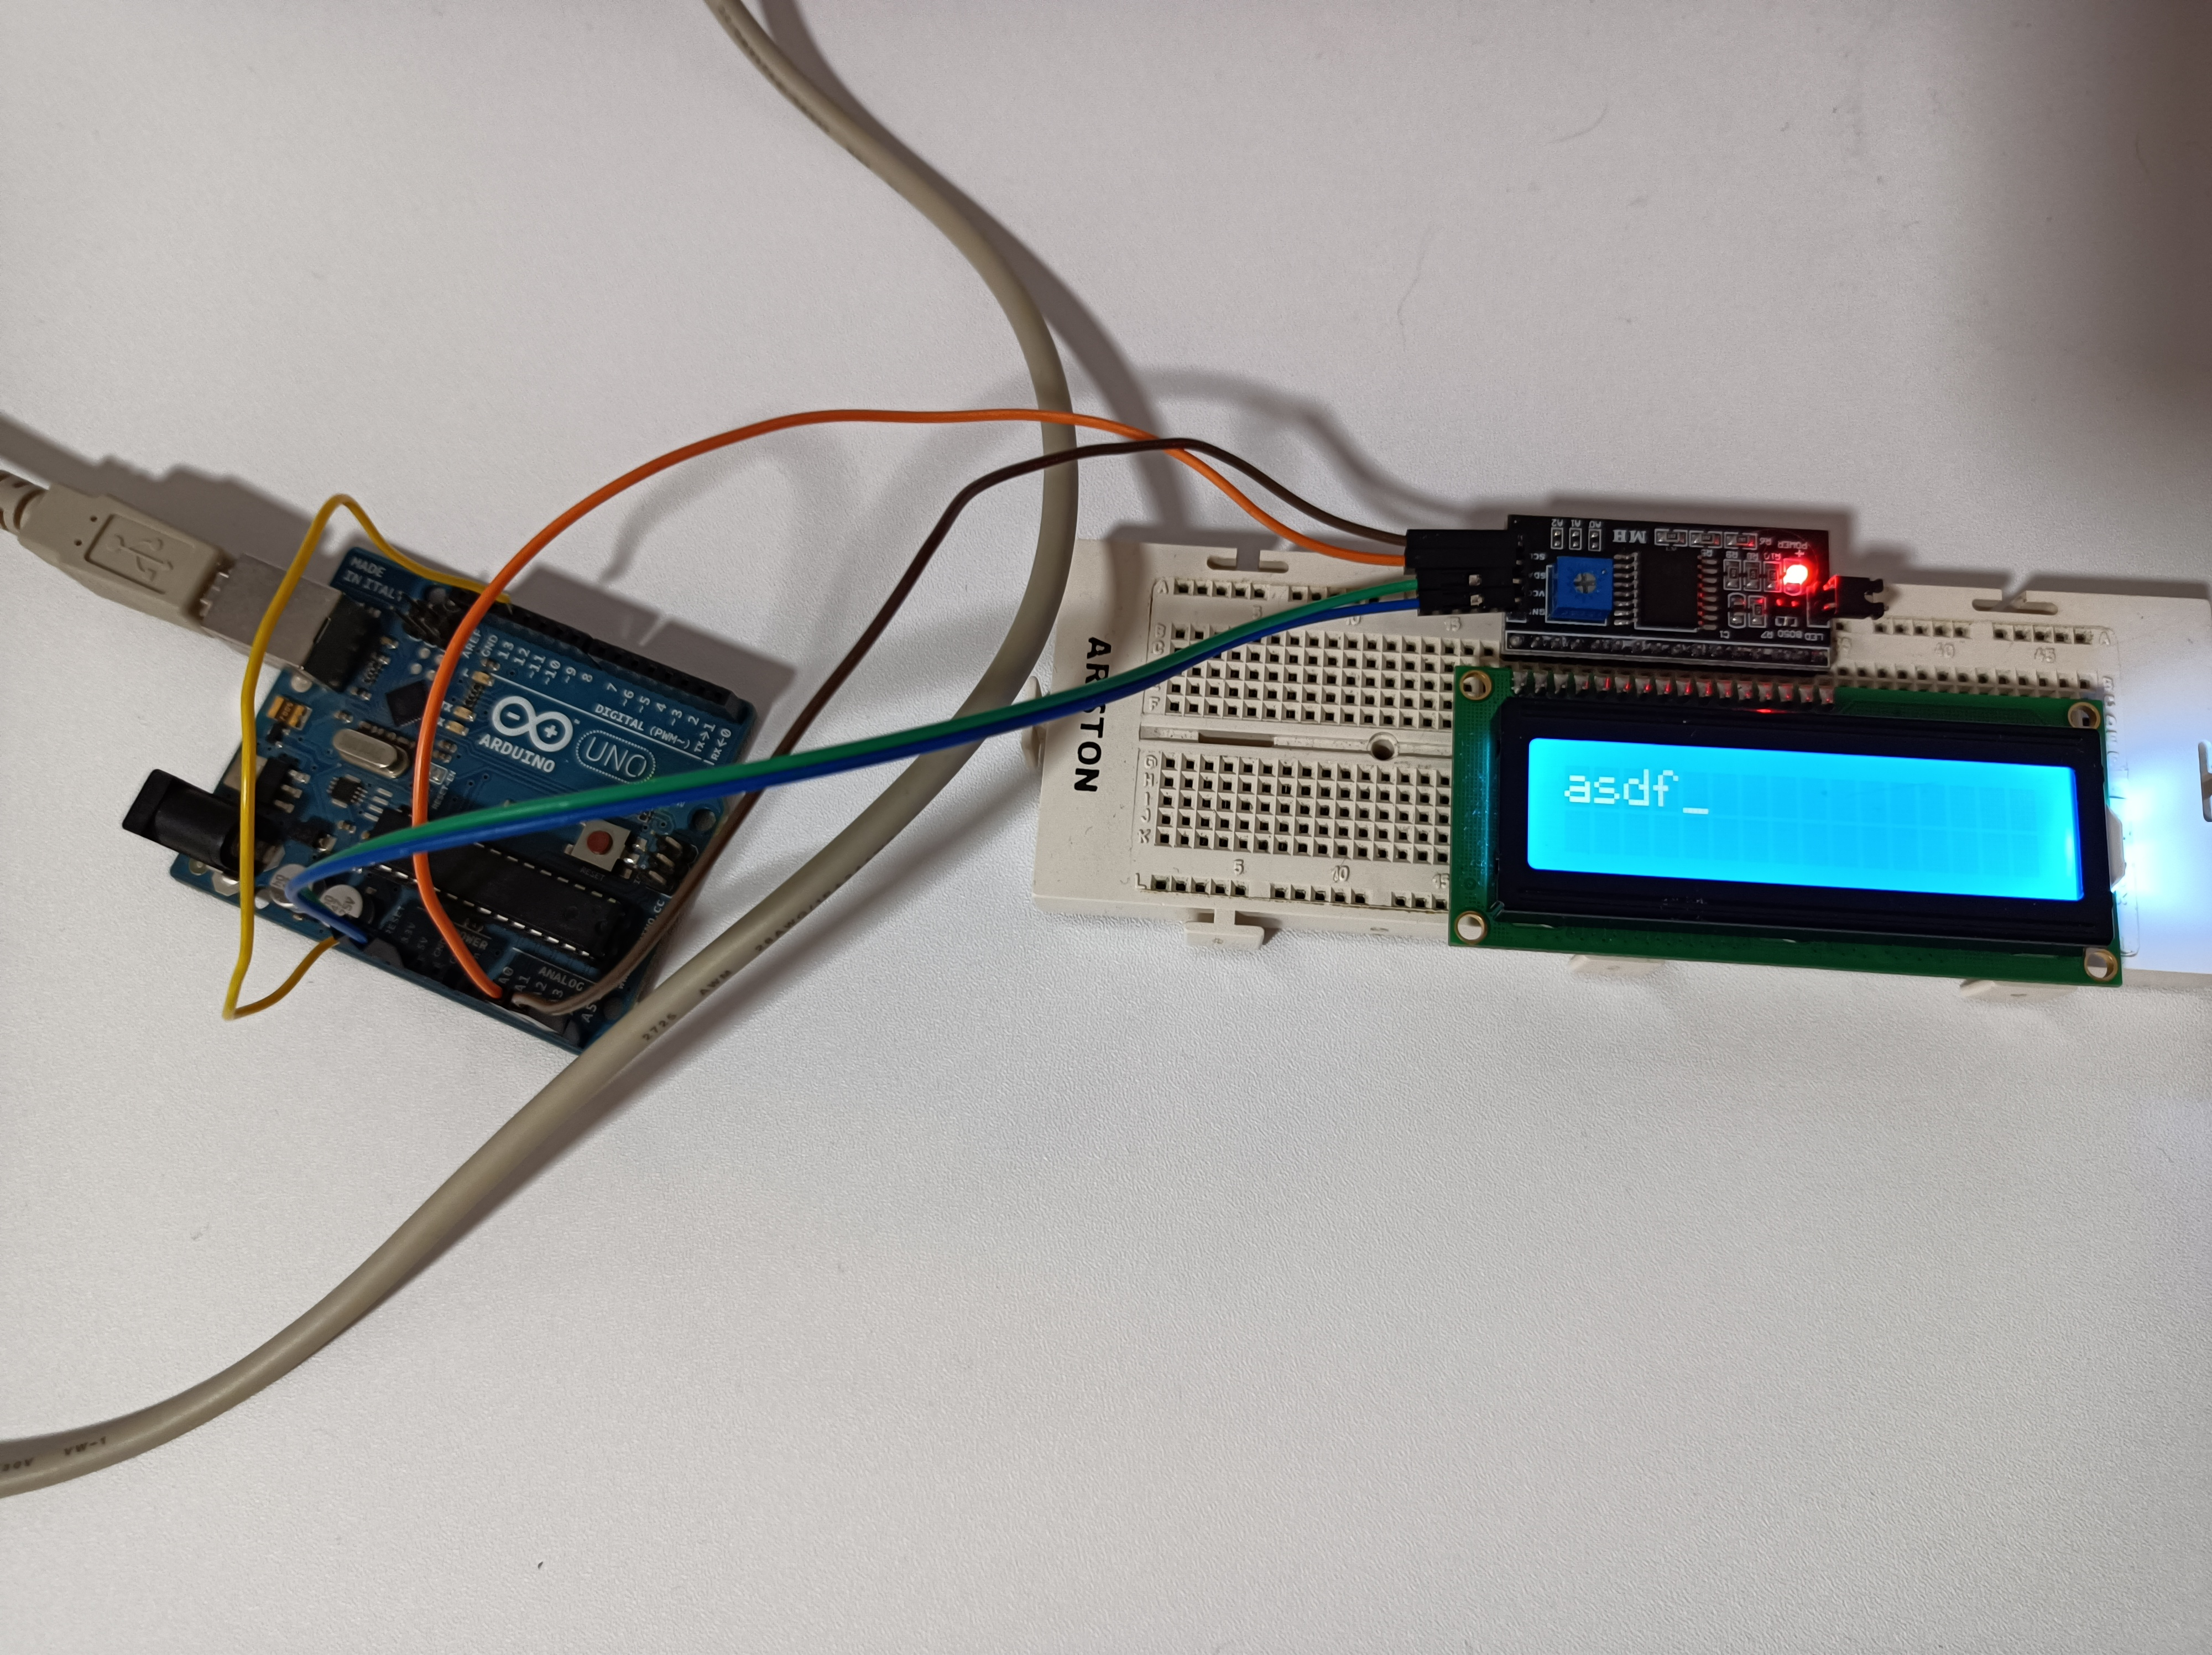
\includegraphics[width=\linewidth]{chars-display-wiring.jpg}

Usaremos una librería que gestiona por nosotros la comunicación con el display
a través del bus I2C. Solo nos queda reenviar los datos recibidos al driver del
LCD:

\lstinputlisting[language=C++, caption=chars-display.ino]{
    1/chars-display/chars-display.ino
}

La aplicación cliente tiene una pequeña complicación, y es que no puede
cerrarse con la pulsación de una tecla. La forma más sencilla es aprovechar
el mecanismo de señal de cierre del sistema operativo, el cual emite dicho
mensaje a la aplicación al presionar la combinación de teclas \verb|Ctrl-C|.
Podemos acceder a esta funcionalidad con la librería \verb|ctrlc|. Llamaremos
al proyecto \verb|chars-display|.

\lstinputlisting[caption=chars-display/Cargo.toml]{
    1/chars-display/Cargo.toml
}

El código de la aplicación cliente se vuelve así muy sencillo:

\lstinputlisting[language=Rust, caption=chars-display/src/main.rs]{
    1/chars-display/src/main.rs
}